\documentclass{classes/SIT-Report-EN}
\usepackage{tabularx}
\usepackage{graphicx}
\usepackage{adjustbox}
\usepackage{lscape}
\usepackage{longtable}
\usepackage{tabularray}
\usepackage{color}
\usepackage{multirow}
\usepackage{graphicx}
\usepackage[normalem]{ulem}
\usepackage{hyperref}
\usepackage{filecontents}
\usepackage{needspace}
\usepackage{array}
\useunder{\uline}{\ul}{}
 
%%Edit your info Here
\begin{document}
\title{LOSTNFOUND KMUTT: KEEP A CLOSE EYES ON YOUR ITEMS.}
\titleTH{ลอสท์แอนด์ฟาวด์ มจธ.}
\degree{Bachelor of Science}
\majorProgramEN{Computer Science}
\academicyear{2024}

\author{MR.PASSAKORN PUTTAMA}
\authorTwo{MR.VATCHARAMAI RODRING}
\authorThree{MR.PATTHADOL RAKSAPRAM}

\majoradvisor{Asst.Prof. Worarat Krathu Ph.D}
\committeeOne{Dr. Watanyoo Suksa-ngaim Ph.D}
\committeeTwo{Dr. Vithida Chongsuphajaisiddhi Ph.D}
\academicyear{2024}

%%%%%%%%%%
\maketitle
\frontmatter
\maketitleinner
\makeapproval
\input{pages/abstract} %%Edit your Abstract
\input{pages/acknowledgements} %% %%Edit your Acknowledgement

\tableofcontents
\listoftables
\listoffigures
%\input{pages/symbols}
%\input{pages/abbreviations}

\mainmatter
%%insert your content
\input{chapter1/chapter1}
\chapter{Feasibility Study}

\section{Introduction}
The LostNFound platform is a centralized web application designed to address the challenges associated with managing lost-and-found items at King Mongkut's University of Technology Thonburi (KMUTT). The platform aims to provide students, staff, and university personnel with an efficient, accessible, and secure solution for reporting and reclaiming lost items.

Unlike the current manual and on-site processes, the LostNFound platform digitizes the entire lost-and-found workflow. Users can report lost items, search for them, and claim ownership through the platform, reducing time and effort. It also introduces features such as real-time item status updates, secure ownership verification, and centralized database management. This initiative aligns with KMUTT’s commitment to modernizing student services and fostering a more convenient university experience.

\section{Problem Statement}
Currently, KMUTT’s lost-and-found system relies on physical reporting to either nearby security personnel or the Student Affairs Division. This approach is inefficient, time-consuming, and prone to security risks such as unauthorized claims. The lack of a unified system makes tracking and managing lost items cumbersome for both users and staff. Furthermore, the absence of a centralized database means there is no effective way to ensure transparency or accessibility for all stakeholders.

The LostNFound platform aims to resolve these issues by providing a digital solution. The platform will centralize all lost-and-found operations, improve communication between stakeholders, and reduce the time required to locate and reclaim lost items. By introducing advanced features such as user profiles, secure claims verification, and automated notifications, the system will create a seamless experience for KMUTT’s community.

\section{Related Research and Projects}
\subsection{Lifeguard Lost \& Found}
A system designed to handle lost and found items in public spaces like airports and transport hubs, which shares similarities with the university setting. It allows users to report, search for, and claim items, ensuring secure ownership verification.

\subsection{MissingX}
A centralized platform for lost and found items, focusing on automatic matching of lost and found property. The platform also supports user notifications when a match is made, aligning with this system’s goal of real-time updates and seamless matching.

\subsection{ItemFinder}
Designed specifically for institutions like universities, ItemFinder handles lost and found items by providing a centralized platform for reporting, cataloging, and verifying items.

\subsection{Comparison of Existing Functions}
\begin{table}[h!]
\centering

\begin{tabular}{|l|p{1.7cm}|p{1.7cm}|p{2cm}|p{1.7cm}|p{1.7cm}|}
\hline
\textbf{Applications} & \textbf{Item Reporting} & \textbf{Matching (NLP)} & \textbf{Notifications} & \textbf{History of Claims} & \textbf{User Profiles} \\
\hline
Lifeguard Lost \& Found & Yes & No & No & No & No \\
\hline
MissingX & Yes & Yes & Yes & No & No \\
\hline
ItemFinder & Yes & No & No & No & Yes \\
\hline
LostNFound KMUTT & Yes & Yes & Yes & Yes & Yes \\
\hline
\end{tabular}
\caption{Existing Functions of Related Applications}
\end{table}

\section{Requirement Specifications}
\subsection{Functional Requirements}
\begin{enumerate}
    \item Report lost and found items by filling out a form with details such as item description, location, and time.
    \item Provide real-time updates regarding the status of items.
    \item Use Natural Language Processing (NLP) to match descriptions of lost and found items.
    \item Notify users when a match is found for their lost item or when their claimed item is ready for pickup.
    \item Maintain a history of claimed items, including photos and verification details.
    \item Integrate with the university’s email system (OAuth with Microsoft) for authentication and ownership verification.
\end{enumerate}

\subsection{Data Requirements}
\begin{enumerate}
    \item \textbf{User Information:} Collect and store user details (e.g., phone number, university email, profile information, claim history) for authentication and personalized user experience.
    \item \textbf{Item Information:} Store details of each lost and found item, including item type, description, location, date, and images.
\end{enumerate}

\section{Implementation Techniques}
\subsection{Frontend}
\begin{itemize}
    \item Programming Language: TypeScript.
    \item Framework: Next.js.
\end{itemize}

\subsection{Backend}
\begin{itemize}
    \item Programming Language: TypeScript, Python.
    \item Frameworks: Next.js, FastAPI.
\end{itemize}

\subsection{Infrastructure}
\begin{itemize}
    \item OS: Debian Linux.
    \item Cloud Provider: Google Cloud Platform (GCP).
    \item Containerization: Docker.
    \item CI/CD: Google Cloud Build.
    \item Deployment Platform: Google Cloud Run.
\end{itemize}

\subsection{Database}
\begin{itemize}
    \item Database Type: Relational (PostgreSQL).
\end{itemize}

\subsection{Testing}
\begin{itemize}
    \item Unit Testing: Jest.
    \item API Testing: Postman.
\end{itemize}

\section{Implementation Plan}
\begin{table}[h!]
\centering
\begin{tabular}{|l|p{5cm}|c|c|c|}
\hline
\textbf{No.} & \textbf{Task Name} & \textbf{Duration} & \textbf{Start Date} & \textbf{End Date} \\ \hline
\multicolumn{5}{|c|}{\textbf{Phase 1: Project Initiation}} \\ \hline
1 & Conduct feasibility study & 10 Days & 15 July 2024 & 24 July 2024 \\ \hline
2 & Define user requirements & 10 Days & 15 July 2024 & 24 July 2024 \\ \hline
3 & Identify technical solutions & 10 Days & 15 July 2024 & 24 July 2024 \\ \hline
4 & Develop project scope and timeline & 10 Days & 15 July 2024 & 24 July 2024 \\ \hline
\multicolumn{5}{|c|}{\textbf{Phase 2: System Architecture Design}} \\ \hline
1 & Define system architecture (Frontend \& Backend) & 10 Days & 25 July 2024 & 3 August 2024 \\ \hline
2 & Design database schema (PostgreSQL) & 10 Days & 25 July 2024 & 3 August 2024 \\ \hline
3 & Design user authentication flow (NextAuth.js) & 10 Days & 25 July 2024 & 3 August 2024 \\ \hline
4 & Define text similarity and matching logic (FastAPI) & 1 Week & 4 August 2024 & 10 August 2024 \\ \hline
\multicolumn{5}{|c|}{\textbf{Phase 3: Development}} \\ \hline
1 & Setup project repository \& development environment (Docker, GCP) & 1 Week & 11 August 2024 & 17 August 2024 \\ \hline
2 & Develop frontend (Next.js + Tailwind CSS) & 2 Weeks & 18 August 2024 & 31 August 2024 \\ \hline
3 & Develop backend API (FastAPI for matching \& item processing) & 2 Weeks & 18 August 2024 & 31 August 2024 \\ \hline
4 & Integrate PostgreSQL database with backend & 2 Weeks & 4 September 2024 & 18 September 2024 \\ \hline
5 & Implement user authentication (OAuth/Microsoft ID) & 2 Weeks & 4 September 2024 & 18 September 2024 \\ \hline
6 & Implement matching logic (NLP, Text Similarity) & 2 Weeks & 4 September 2024 & 18 September 2024 \\ \hline
7 & Setup notifications & 3 Days & 19 September 2024 & 21 September 2024 \\ \hline
\multicolumn{5}{|c|}{\textbf{Phase 4: Testing}} \\
\hline
1 & Conduct unit tests (Frontend and Backend) & 1 Week & 22 September 2024 & 28 September 2024 \\
\hline
2 & Perform integration testing (Frontend + Backend) & 4 Weeks & 1 October 2024 & 30 October 2024 \\
\hline
\multicolumn{5}{|c|}{\textbf{Phase 5: Deployment Preparation}} \\
\hline
1 & Prepare deployment environment on Google Cloud & 2 Days & 30 October 2024 & 31 October 2024 \\
\hline
2 & Prepare deployment environment on Google Cloud & 2 Days & 1 November 2024 & 2 November 2024 \\
\hline
\multicolumn{5}{|c|}{\textbf{Phase 6: Deployment}} \\
\hline
1 & Deploy the application to Google Cloud using Cloud Run & 4 Days & 4 November 2024 & 8 November 2024 \\
\hline
\end{tabular}
\caption{Implementation Plan}
\end{table}


\chapter{SYSTEM ANALYSIS AND DESIGN}

\section{Introduction}
\par
This chapter provides an explanation of our project design in the following sections: analysis of the existing system, diagram, system architecture, system design, and user interface design.

\section{Analysis of the existing system}
\par
The scope of this project is centered on King Mongkut’s University of Technology Thonburi (KMUTT) as the designated target area. The primary user groups are the personnel within the organization.

\section{User Requirement Analysis}
\subsection{User Requirements}
\par
The following are the functional specifications that users expect from the LostNFound KMUTT platform:
\begin{enumerate}
    \item \textbf{Lost and Found Item Reporting:} The system should allow users (students and university staff) to report lost and found items. Users should be able to submit detailed descriptions for the items they are reporting. This information is essential for accurate matching.
    \item \textbf{Item Matching:} The platform should use advanced text-matching techniques, such as Natural Language Processing (NLP), to compare lost and found item descriptions and ensure the correct matching between them. This allows users to easily identify and claim their belongings.
    \item \textbf{Secure Claim Process:} The system must verify users' identities using their \textbf{university email} to ensure only the rightful owner can claim an item. The platform should reject any claims from users who cannot prove ownership of the lost item.
    \item \textbf{History of Claimed Items:} The system needs to maintain a detailed record of all claimed items, including the name and ID of the user who claimed the item. This helps provide accountability and keeps a history of item claims for future reference.
    \item \textbf{Notification System:} Users should receive timely notifications when a match is found for their lost item or when they are reminded to pick up an item they have claimed.
    \item \textbf{Authentication and Security:} The system must ensure secure authentication using \textbf{Microsoft Extra ID} to authenticate users. Only users with valid \textbf{KMUTT email accounts} should be able to access the platform and participate in reporting or claiming items.
\end{enumerate}

\section{System design}
\subsection{Proposed Architecture Diagram}
\begin{figure}[!h]
    \centering
    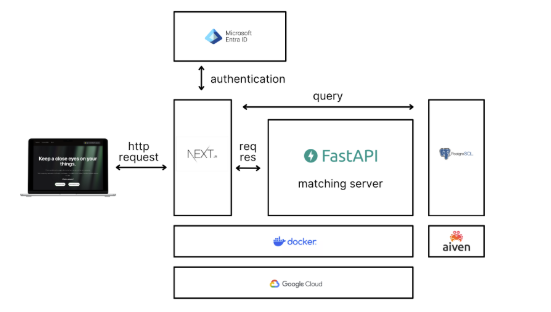
\includegraphics[width=1\linewidth]{chapter3/architecture-diagram.png}
    \caption{Architecture Diagram}
    \label{fig:Architecture Diagram}
\end{figure}
\par Figure 3.1 represents our system architecture. The platform will leverage Google Cloud Platform (GCP) for hosting, with Cloud Registry used for storing Docker images, and Cloud Build for automating the build process. The application will run on Cloud Run, providing a serverless environment for deploying containerized applications. For frontend development, we will use Next.js with Tailwind CSS for responsive and stylish web pages. The backend will be developed with FastAPI, which will expose NER and Text Similarity APIs for matching lost and found items. PostgreSQL will be used for storing data related to users and items, hosted on Aiven for managed database services. Docker will be utilized for containerizing the entire application, enabling efficient deployment and scalability within the cloud environment.

\newpage
\subsection{Context Diagram}
\begin{figure}[!h]
    \centering
    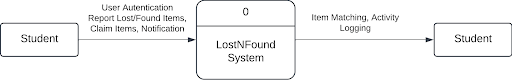
\includegraphics[width=1\linewidth]{chapter3/context-diagram.png}
    \caption{Context Diagram of LostNFound System}
    \label{fig:Context Diagram of LostNFound System}
\end{figure}
\par This figure shows the context diagram for the LostNFound KMUTT system. The diagram illustrates the overall interactions between the users and the system. Users (students and staff) are required to authenticate via their KMUTT email to access the platform. Once authenticated, students can report lost and found items. The core interactions of the system include the submission of item reports, matching items using \textbf{Text Similarity and NER APIs}, and the ability for users to track and claim their lost belongings.

\subsection{Data Flow Diagram}
\begin{figure}[!h]
    \centering
    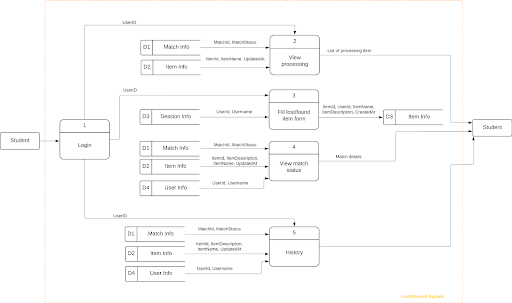
\includegraphics[width=1\linewidth]{chapter3/data-flow-diagram.png}
    \caption{Diagram 0}
    \label{fig:Diagram 0}
\end{figure}
\par
Figure 3.3 represents the data flow diagram of the LostNFound KMUTT system. The process starts when the user inputs their KMUTT email and password to authenticate. Once authenticated, the user can report a lost or found item by providing item details, such as description, location, and timestamp. The system processes and stores the data in the PostgreSQL database. Users can then view item matches using NLP for text similarity, claim found items, and receive notifications when a match is found or when they need to pick up their claimed item.

\newpage
\subsection{Activity Diagram}
\begin{figure}[!h]
    \centering
    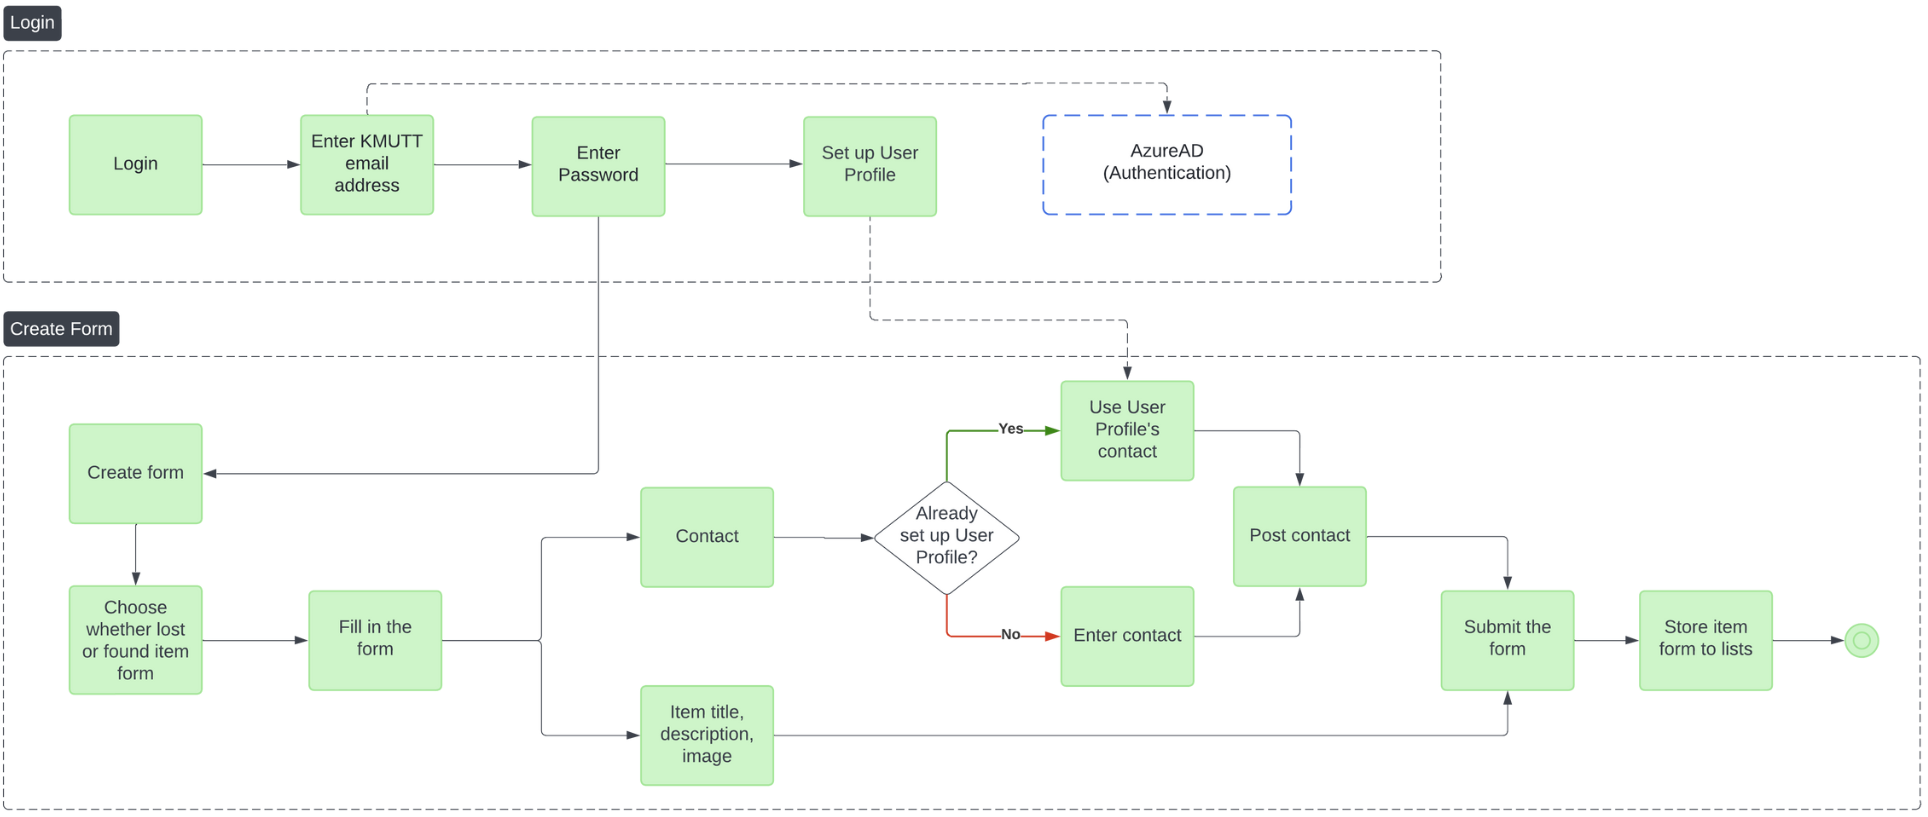
\includegraphics[width=1\linewidth]{chapter3/activity-diagram.png}
    \caption{Activity Diagram for student logins and creating lost or found item form of LostNFound System}
    \label{fig:Activity Diagram for student logins and creating lost or found item form of LostNFound System}
\end{figure}
\par
Figure 3-4 represents the flow when the student uses a web application by logging in with Microsoft Extra ID authentication. Once authenticated, the student is directed to the form page where they can choose to create a lost item or found item form. The student fills in the required details, including the item description. After submission, the form data is processed and stored in the system, where it can be used for matching with other lost or found items.

\newpage
\begin{figure}[!h]
    \centering
    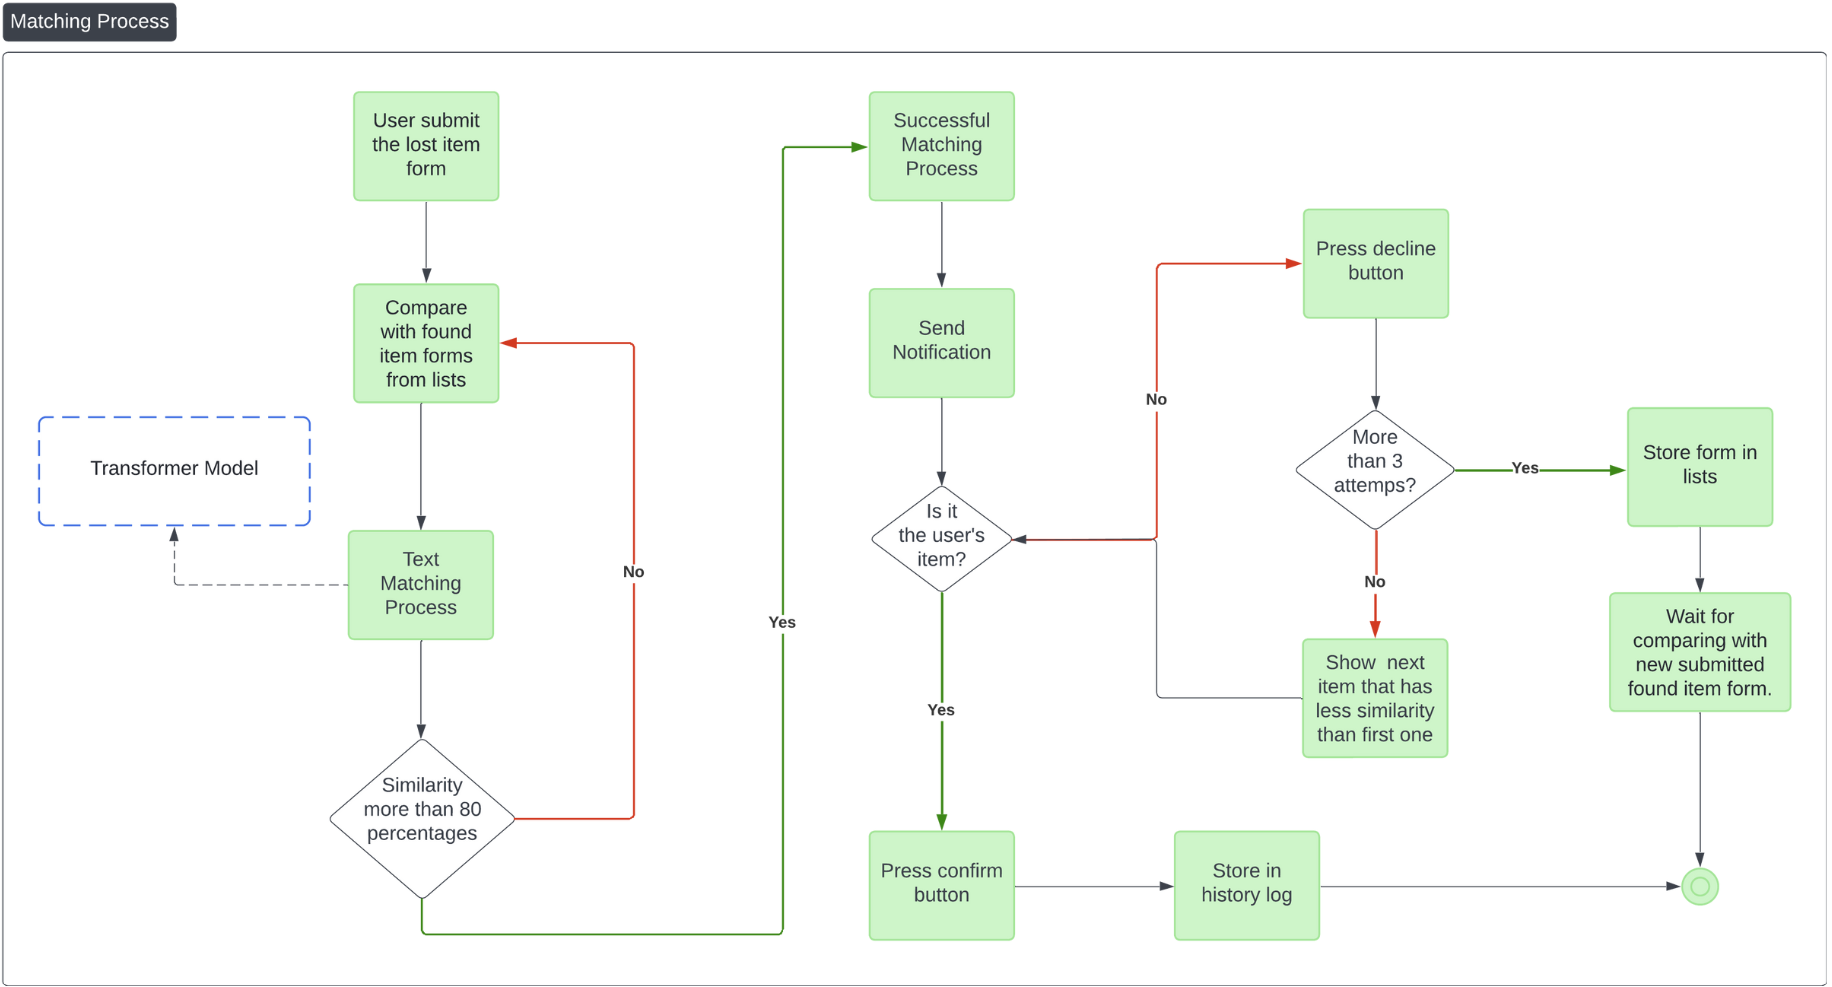
\includegraphics[width=1\linewidth]{chapter3/activity-diagram2.png}
    \caption{Activity Diagram for a matching process of LostNFound System}
    \label{fig:Activity Diagram for a matching process of LostNFound System}
\end{figure}
\par
Figure 3.5 represents the matching process in the LostNFound KMUTT system. The process begins when a lost item report or a found item report is submitted by a student or staff member. Once the report is submitted, the system uses Natural Language Processing (NLP) and Text Similarity algorithms to compare the item descriptions. The system processes key details such as description, product name, and location to identify potential matches.

\newpage
\begin{figure}
    \centering
    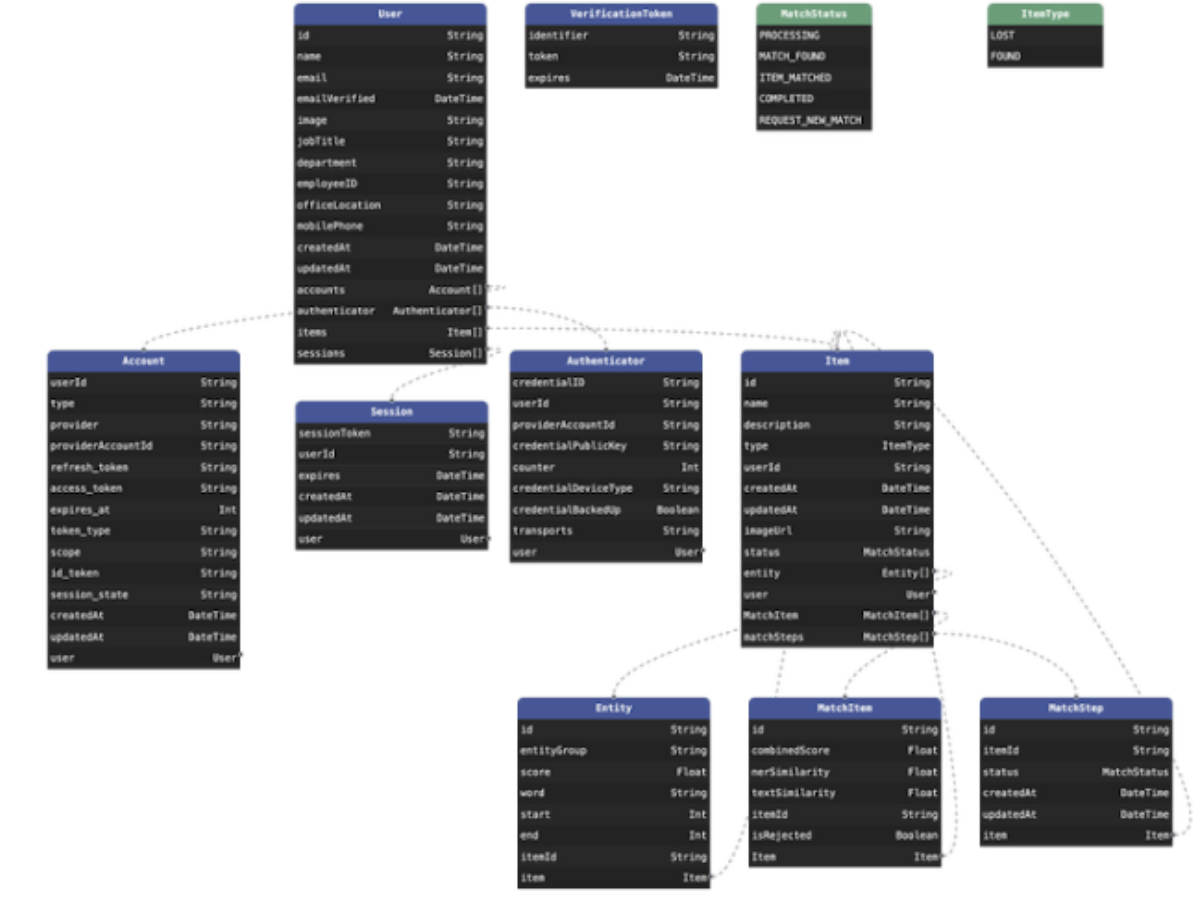
\includegraphics[width=1\linewidth]{chapter3/er-diagram.png}
    \caption{ER Diagram of LostNFound System}
    \label{fig:ER Diagram of LostNFound System}
\end{figure}
\par
Figure 3.6 represents the conceptual diagram of the LostNFound System which we will use to store information about users and match details.
\input{chapter4/chapter4}
\input{chapter5/chapter5}

\bibliographystyle{plain}
\bibliography{references/references}
% \cite{gcp2023}
% \cite{huggingface2023}
% \cite{fastapi2022}
% \cite{nextjs2023}

\end{document}